\section{Classical Calculations}

\begin{frame}
\frametitle{Classical DFT Approach}
\begin{itemize}
    \item Periodic DFT calculations using CP2K
    \item System: Al(111) surface with triazole inhibitor
    \item Geometry optimization using ML potentials
\end{itemize}
\end{frame}

\begin{frame}
\frametitle{Case Study: Corrosion Inhibition}
\begin{itemize}
    \item Study of 1,2,4-triazole molecule on Al(111) surface
    \item Focus on metal-inhibitor interaction
    \item Goal: Calculate binding energy accurately
\end{itemize}
\end{frame}

\begin{frame}
\frametitle{System Setup}
\begin{columns}
\column{0.5\textwidth}
\begin{itemize}
    \item 4×4 Al(111) supercell
    \item PBE functional with D3 dispersion correction
    \item DZVP-MOLOPT-GTH basis sets
\end{itemize}
\column{0.5\textwidth}
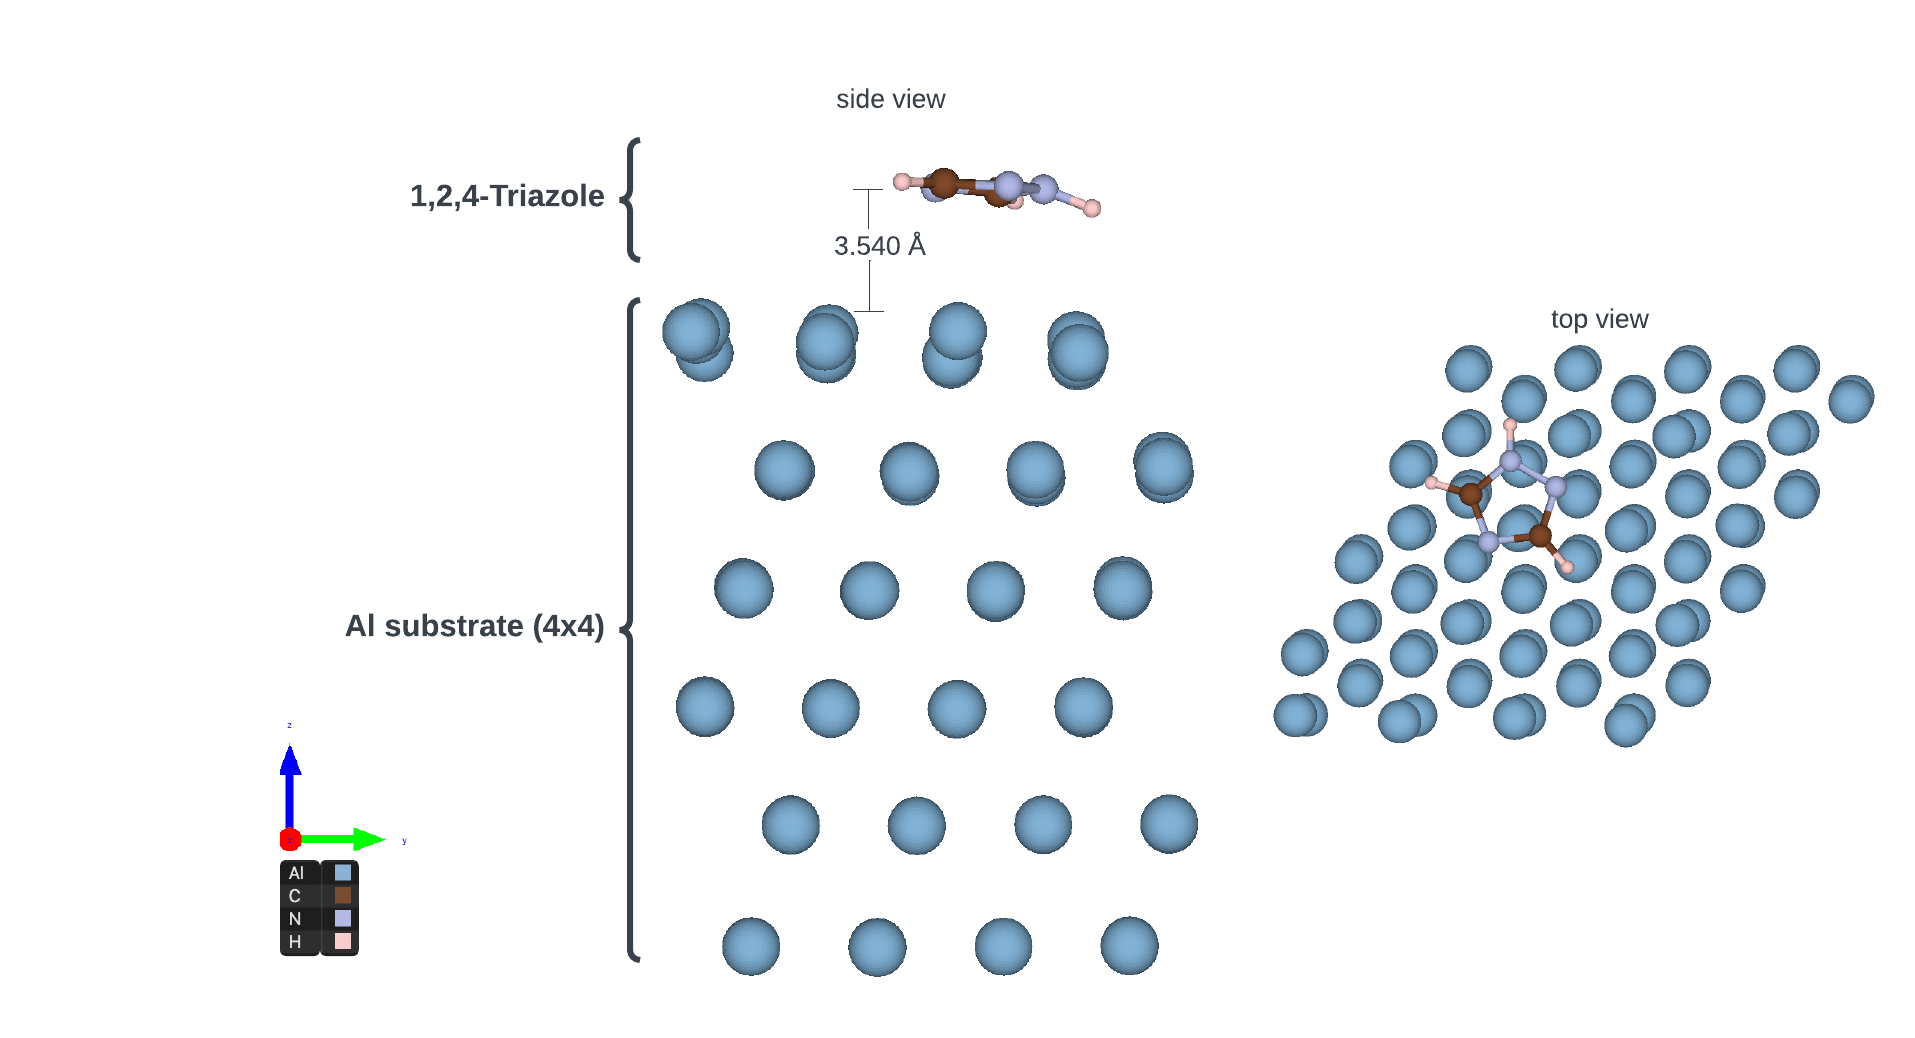
\includegraphics[width=\textwidth]{../../../content/img/workflow_viz1.png}
\end{columns}
\end{frame}

\begin{frame}
\frametitle{Computational Details}
\begin{itemize}
    \item GPW method (500 Ry plane-wave cutoff)
    \item Periodic boundary conditions with 25 Å vacuum gap
    \item Fermi-Dirac distribution (1000 K electronic temperature)
    \item DFT-D3 dispersion correction for van der Waals interactions
\end{itemize}
\end{frame}

\begin{frame}
\frametitle{Workflow Steps}
\begin{enumerate}
    \item Supercell generation with ASE
    \item Geometry optimization with ML potentials
    \item DFT calculations for periodic system
    \item Binding energy calculation:
    \[ E_{\text{binding}} = E_{\text{supercell}} - (E_{\text{substrate}} + E_{\text{inhibitor}}) \]
\end{enumerate}
\end{frame} 